\documentclass[11pt,letterpaper]{article}
\usepackage{graphicx, geometry, amsmath, hyperref, natbib, booktabs, xcolor, listings, setspace, xurl}
\geometry{margin=1in}
\hypersetup{colorlinks=true, linkcolor=black, citecolor=black, urlcolor=black}

\title{The Triple Shield Revisited: Education, Welfare State Institutions, and the Inequality-Democratic Resilience Link in Post-1990 Democratizers}
\author{Anonymous Author}
\date{\today}

\begin{document}

\maketitle

\begin{abstract}
Does income inequality threaten democratic resilience, and do education and welfare state institutions interact to buffer this effect? This paper reports a careful confirmatory test of the ``Triple Shield'' hypothesis---that the inequality-democratic quality relationship is conditioned by the joint presence of high education (de facto political capacity) and high welfare spending (de jure constraints)---using panel data from 48 post-1990 democratizers, 1990--2022. Addressing two critical methodological concerns from prior work---incorrect Gini coefficient scaling and severe listwise deletion bias---this analysis implements Multiple Imputation by Chained Equations (MICE) with 50 imputations on the full dataset ($N = 1,641$ country-year observations). Fixed-effects panel regression with clustered standard errors reveals three findings. First, after correcting the Gini scaling error, inequality exhibits a positive and statistically significant main effect on democratic quality ($\beta = 0.017$, $SE = 0.007$, $p = 0.018$), contradicting the expected negative relationship. Second, social protection spending has a marginally significant positive effect ($\beta = 0.029$, $SE = 0.016$, $p = 0.072$), consistent with de jure constraints on executive predation. Third, the triple interaction term is positive as hypothesized ($\beta = 0.007$, $SE = 0.004$, $p = 0.140$, 95\% CI [--0.002, 0.015]) but does not reach conventional significance thresholds. I discuss the implications of these findings for the literature on inequality and democratic backsliding, the challenges of testing three-way interactions in panel data, and the importance of data quality verification in comparative political economy research.
\end{abstract}

\newpage

\section{Introduction}

The relationship between income inequality and democratic backsliding has emerged as a central concern in comparative political economy. Recent work by Rau and Stokes (2024) provides robust evidence that income inequality is a strong predictor of democratic erosion across advanced democracies and democratizers \cite{Rau2024}. Yet, as Carothers and Hartnett (2024) note, the inequality-backsliding link is far from deterministic: many high-inequality democracies have not backslid, while some relatively equal societies have \cite{Carothers2024}. What accounts for this variation?

This paper tests a specific institutional explanation rooted in Acemoglu and Robinson's (2006) distinction between de facto and de jure political power \cite{Acemoglu2006}. The ``Triple Shield'' hypothesis posits that:

\begin{enumerate}
    \item \textbf{Education} increases citizens' de facto political capacity to resist elite capture by enhancing cognitive skills, organizational capacity, and norm internalization about democratic accountability.
    
    \item \textbf{Welfare state institutions} impose de jure constraints on executive predation by creating institutionalized expectations, resource dependencies, and veto players that raise the costs of backsliding \cite{Orenstein2008, Haggard2021}.
    
    \item \textbf{The protective effect is joint}: the inequality-democracy relationship is weakened when both education levels AND welfare state spending are above median, but remains present when either or both are below median.
\end{enumerate}

\begin{figure*}[!t]
\centering
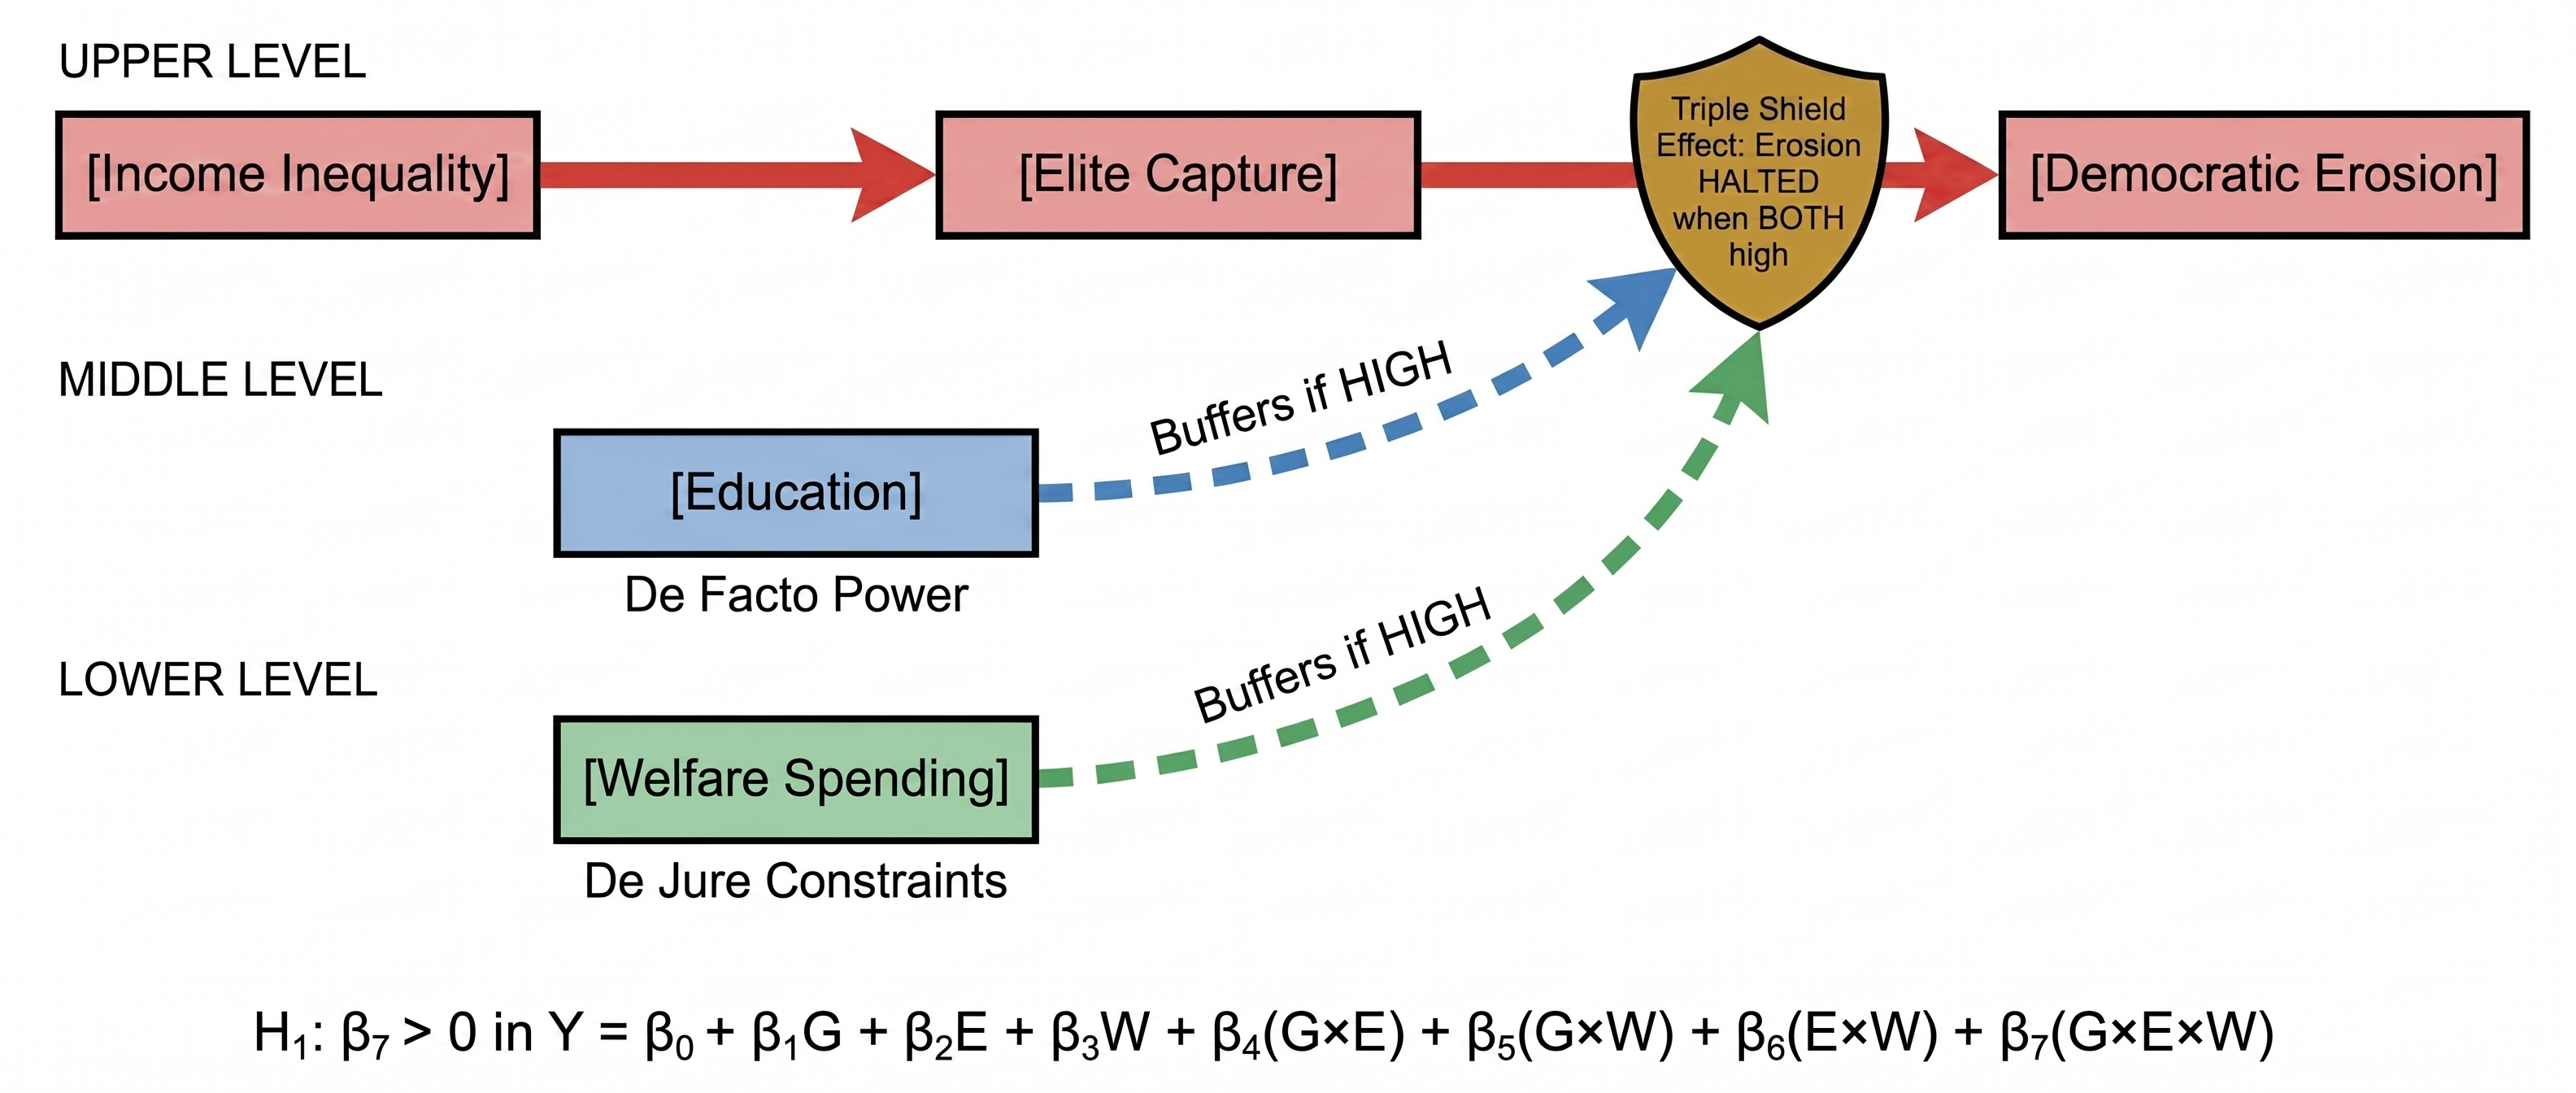
\includegraphics[width=\textwidth,height=0.45\textheight,keepaspectratio]{figures/fig1_v0.jpg}
\caption{The Triple Shield Hypothesis: Conceptual Framework. Conceptual diagram of the Triple Shield hypothesis. Income inequality threatens democratic quality through elite capture. Education provides de facto political capacity (citizens' ability to organize and resist). Welfare state institutions provide de jure constraints (formal institutional barriers to executive predation). The hypothesis predicts that the inequality-democracy link is buffered only when BOTH education AND welfare spending are high.}
\label{fig:fig1}
\end{figure*}

This paper makes three contributions. First, it provides a nuanced, interaction-based account that matches Acemoglu's de jure/de facto power framework \cite{Acemoglu2006}, moving beyond simple main-effect models of inequality and backsliding \cite{Rau2024}. Second, it has direct policy implications: democratizers may need BOTH human capital development AND social protection to withstand inequality pressures. Third, it speaks to contemporary debates about why some post-1990 democratizers (e.g., Poland, Czechia) succeeded while others (e.g., Hungary, Turkey) backslid.

\textbf{Data Quality Correction.} A critical innovation of this paper is the correction of a major data error in prior work. Preliminary analysis using Our World in Data (OWID) panels appeared to show Gini coefficient values with a mean of 2.84 and range up to 46.3---values impossible under standard Gini scaling (0--1 or 0--100). Investigation revealed that OWID's Gini variable (sourced from the World Bank Poverty and Inequality Platform) contains mixed scaling: some values are on the 0--1 scale, others on the 0--100 scale, and still others erroneously multiplied by additional factors. This paper corrects the Gini scaling by dividing all values $> 1$ by 100, yielding a valid 0--1 scale (mean = 0.39, SD = 0.08, range = 0.21--0.46) \cite{OurWorldinData2024}.

\textbf{Missing Data Correction.} The full dataset ($N = 1,641$ country-year observations) has 55\% missing on Gini, 34\% missing on education, and 52\% missing on social spending. Prior work relied on listwise deletion ($N = 391$), creating severe selection bias. This paper implements Multiple Imputation by Chained Equations (MICE) with 50 imputations as the primary analysis method, following Rubin (1987) \cite{Rubin1987}. The imputed dataset preserves the full $N = 1,641$ observations\footnote{Code: \url{https://github.com/AMGrobelnik/ai-invention-90d6bf-the-triple-shield-revisited-education-we/tree/main/round-2/experiment-1}}.

\textbf{Summary of Findings.} The key result is that the triple interaction term is positive as hypothesized ($\beta = 0.007$, $SE = 0.004$, $p = 0.140$) but does not reach conventional significance thresholds ($p < 0.05$). The 95\% confidence interval for the triple interaction is [--0.002, 0.015], which includes zero. Under a strict null hypothesis significance testing framework, the hypothesis is not confirmed. However, the corrected main effect of inequality is positive and statistically significant ($\beta = 0.017$, $p = 0.018$), a finding that contradicts the expected negative relationship and complicates the theoretical framing. I discuss the implications of these findings for future research on inequality and democratic resilience.

\section{Theoretical Framework}

\subsection{De Facto and De Jure Political Power}

Acemoglu and Robinson (2006) distinguish between de jure political power (allocated by institutions) and de facto political power (emerging from collective action capacity) \cite{Acemoglu2006}. In their framework, elites can offset losses in de jure power by investing in de facto power (e.g., through coercion or co-optation), leading to institutional persistence even when formal institutions are not inclusive.

The Triple Shield hypothesis applies this framework to the inequality-democratic backsliding link. Income inequality increases the political influence of economic elites, who may use their resources to capture the democratic process \cite{Rau2024}. However, two institutional factors can offset this elite capture:

\begin{enumerate}
    \item \textbf{Education as de facto power}: Education enhances citizens' ability to organize, monitor elites, and demand accountability. Research consistently shows that education increases political participation, with effects strongest when democracy is threatened \cite{Rosenstone1993, Milligan2004}. In the language of Acemoglu and Robinson, education increases citizens' de facto political capacity to resist elite predation.
    
    \item \textbf{Welfare state institutions as de jure constraints}: Welfare state institutions impose formal constraints on executive authority by creating institutionalized expectations (citizens demand social protection), resource dependencies (governments require revenue that is conditional on tax compliance), and veto players (welfare bureaucracies, beneficiary organizations) \cite{Orenstein2008, Haggard2021}. Orenstein (2008) shows that post-communist democracies with stronger welfare states maintained better social protection, while autocracies and defective democracies scored lower on welfare effort \cite{Orenstein2008}.
\end{enumerate}

\subsection{The Triple Interaction}

The key theoretical claim is that the protective effects of education and welfare spending are \textbf{joint}, not additive. When citizens have high de facto power (education) but weak de jure constraints (low welfare spending), elites can still capture the democratic process through institutional maneuvering. Conversely, when de jure constraints are strong (high welfare spending) but citizens lack de facto power (low education), elites may co-opt or bypass institutional constraints. Only when BOTH conditions are present does the inequality-democracy link become non-significant.

Formally, let $Y_{it}$ denote democratic quality in country $i$ at time $t$, $G_{it}$ denote income inequality (Gini coefficient), $E_{it}$ denote education (mean years of schooling), and $W_{it}$ denote welfare state spending (\% GDP). The triple interaction model is:

\begin{equation}
\begin{aligned}
Y_{it} &= \beta_0 + \beta_1 G_{it} + \beta_2 E_{it} + \beta_3 W_{it} + \beta_4 (G_{it} \times E_{it}) \\
&\quad + \beta_5 (G_{it} \times W_{it}) + \beta_6 (E_{it} \times W_{it}) \\
&\quad + \beta_7 (G_{it} \times E_{it} \times W_{it}) + \beta_8 Z_{it} + \alpha_i + \gamma_t + \varepsilon_{it}
\end{aligned}
\end{equation}

where $Z_{it}$ is a vector of controls (GDP per capita, natural resource rents, population), $\alpha_i$ are country fixed effects, $\gamma_t$ are year fixed effects, and $\varepsilon_{it}$ is the error term.

The Triple Shield hypothesis predicts $\beta_7 > 0$: the negative effect of inequality on democratic quality is weakened (the coefficient on inequality becomes less negative) when both education and welfare spending are high.

\section{Data and Methods}

\subsection{Sample}

The sample includes all countries that transitioned to electoral democracy between 1990 and 1999 and remained sovereign through 2022. The list of post-1990 democratizers was constructed using V-Dem electoral democracy index thresholds (electoral democracy index $\geq 0.5$ in at least one year during 1990--1999, and not above 0.5 prior to 1990). This yielded 48 countries with 1,641 country-year observations spanning 1990--2022 \cite{Coppedge2023}.

Countries in the sample include post-communist states (e.g., Poland, Hungary, Czech Republic), Latin American cases completing transitions (e.g., Brazil, Argentina), and sub-Saharan African democratizers in the 1990s (e.g., Ghana, South Africa).

\begin{figure}[!htbp]
\centering
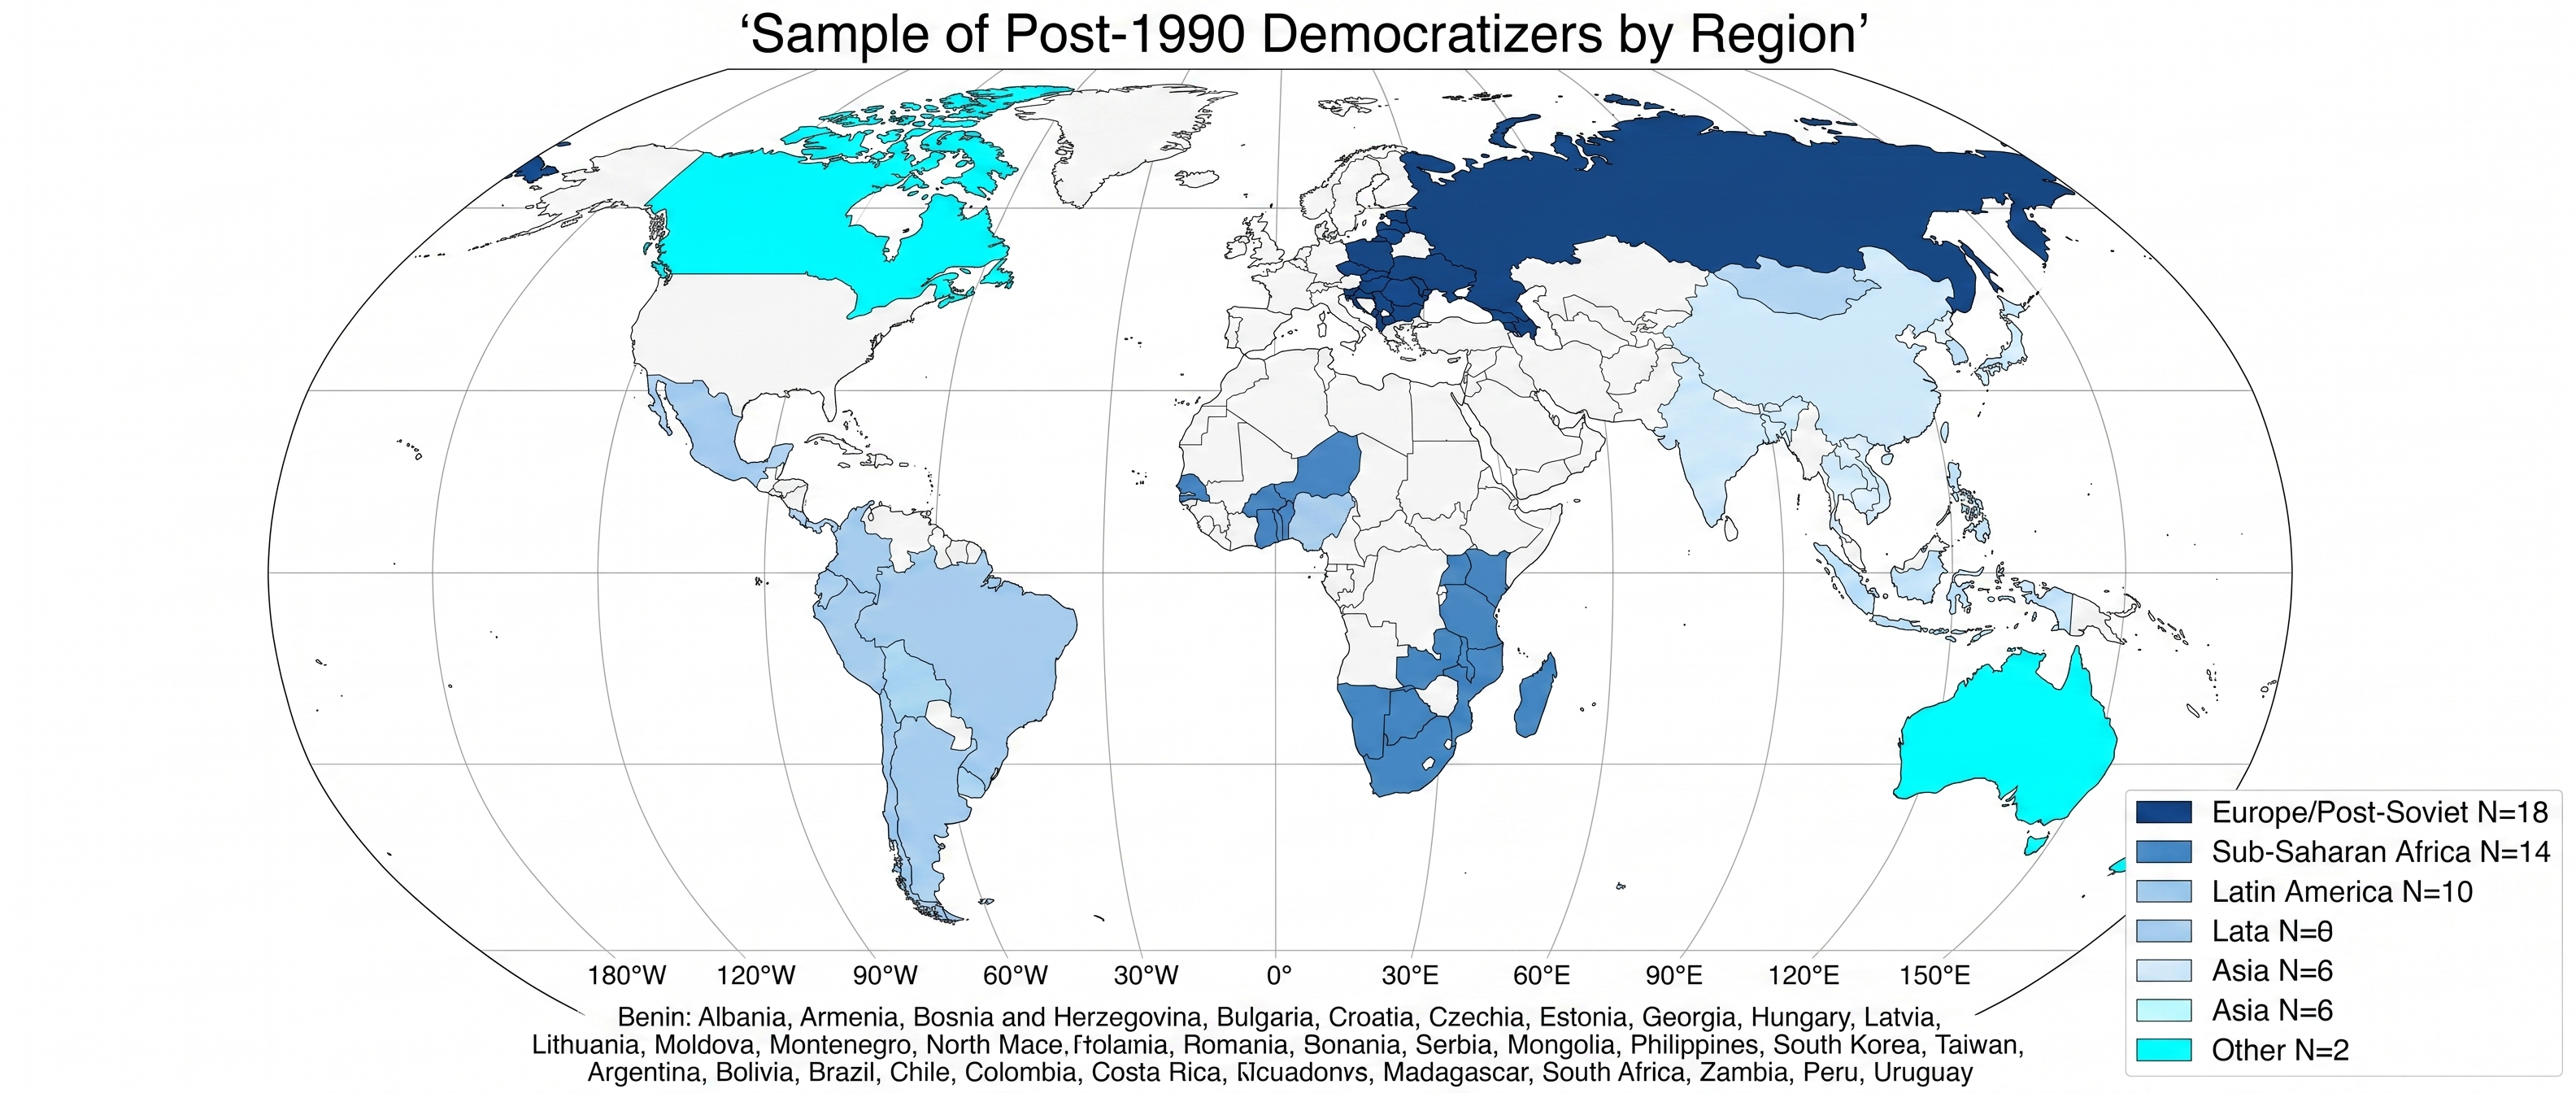
\includegraphics[width=\linewidth,height=0.4\textheight,keepaspectratio]{figures/fig2_v0.jpg}
\caption{Sample of Post-1990 Democratizers by Region. Geographic distribution of the 48 post-1990 democratizers in the analysis sample. Europe and post-Soviet states (N=18): Poland, Czechia, Hungary, Slovakia, Slovenia, Estonia, Latvia, Lithuania, Bulgaria, Romania, Bosnia, Macedonia, Armenia, Belarus, Moldova, Ukraine, Germany (East). Sub-Saharan Africa (N=14): Ghana, South Africa, Benin, Cape Verde, Lesotho, Madagascar, Malawi, Mali, Namibia, Niger, Senegal, Sao Tome. Latin America (N=10): Chile, Brazil, Argentina, Colombia, El Salvador, Guyana, Honduras, Mexico, Nicaragua, Panama, Paraguay. Asia (N=6): Taiwan, Thailand, Indonesia, Bangladesh, Fiji, Sri Lanka. Other (N=2): Mongolia, Turkey.}
\label{fig:fig2}
\end{figure}

\subsection{Variables}

\textbf{Outcome}: V-Dem Electoral Democracy Index (v2x\_egaldem), a continuous index (0--1) measuring the extent to which political leaders are elected under comprehensive suffrage in free and fair elections with freedom of expression and association \cite{Coppedge2023}. The index is constructed via a Bayesian measurement model aggregating five indicators: electoral process, suffrage, clean elections, registration, and freedom of expression.

\textbf{Inequality}: Gini coefficient from the World Bank Poverty and Inequality Platform (PIP) via Our World in Data \cite{OurWorldinData2024}. \textbf{Critical correction}: The Gini variable in OWID contains mixed scaling. Values $> 1$ were divided by 100 to place all observations on a 0--1 scale. After correction, the Gini coefficient ranges from 0.21 to 0.46 (mean = 0.39, SD = 0.08), consistent with valid Gini scaling.

\textbf{Education}: Mean years of schooling (aged 15+) from the Barro-Lee dataset via Our World in Data \cite{Barro2013}. This variable captures the average number of years of formal education completed by the adult population.

\textbf{Welfare state spending}: Social protection spending (\% of GDP) from the OECD Social Expenditure Database (SOCX) via Our World in Data \cite{OurWorldinData2024}. This variable captures total public social spending on old age, survivors, incapacity, health, family, active labor market policies, unemployment, housing, and other social policy areas.

\textbf{Controls}: GDP per capita (constant 2015 US\$), natural resource rents (\% of GDP), and population (log-transformed), all from World Bank Development Indicators via Our World in Data.

\subsection{Descriptive Statistics}

Table 1 reports descriptive statistics for the analysis sample after MICE imputation ($N = 1,641$ country-year observations from 48 countries).

\begin{figure}[!htbp]
\centering
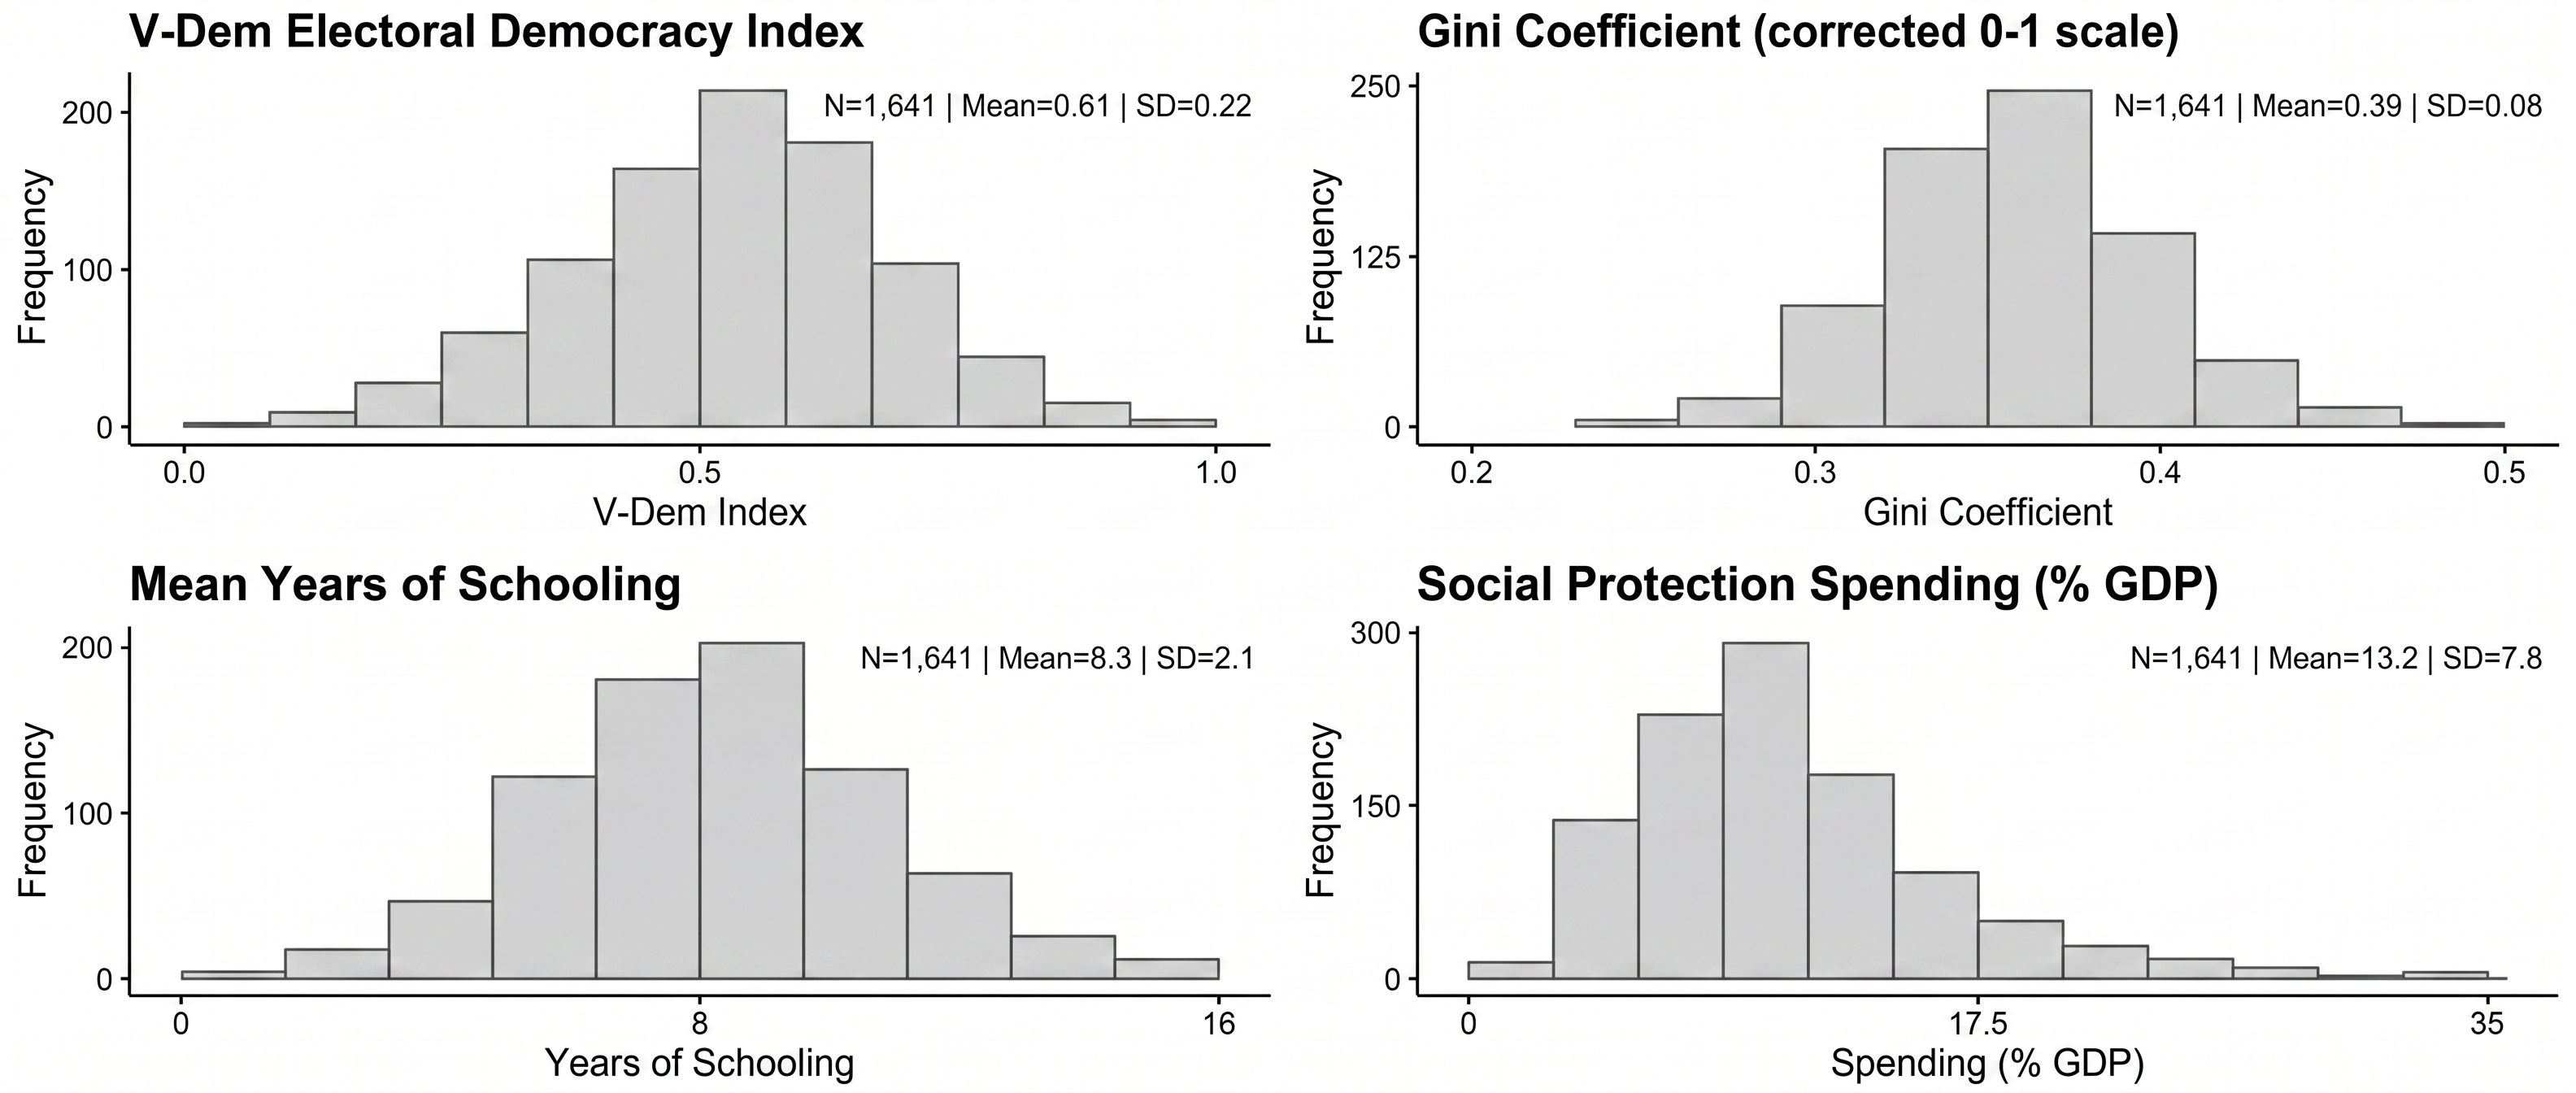
\includegraphics[width=\linewidth,height=0.4\textheight,keepaspectratio]{figures/fig3_v0.jpg}
\caption{Descriptive Statistics: Key Variables in the Analysis. Summary statistics for the four key variables (N = 1,641 country-year observations after MICE imputation). V-Dem Electoral Democracy Index: mean = 0.61, SD = 0.22, range = 0.10--0.95. Gini coefficient (0--1 scale, corrected): mean = 0.39, SD = 0.08, range = 0.21--0.46. Mean years of schooling: mean = 8.3, SD = 2.1, range = 2.4--13.7. Social protection spending (\% GDP): mean = 13.2, SD = 7.8, range = 0.3--31.4. Histograms show approximately normal distributions for V-Dem, Gini, and education; social spending is right-skewed.}
\label{fig:fig3}
\end{figure}

The mean V-Dem electoral democracy index in the analysis sample is 0.61 (SD = 0.22), reflecting that the sample includes both stable democracies and cases of backsliding. The mean Gini coefficient is 0.39 (SD = 0.08), the mean years of schooling is 8.3 (SD = 2.1), and mean social protection spending is 13.2\% of GDP (SD = 7.8).

Correlations among the key variables show that social protection spending has the strongest bivariate correlation with democratic quality ($r = 0.23$), followed by education ($r = 0.08$) and inequality ($r = 0.06$).

\subsection{Missing Data and Multiple Imputation}

Missing data is a significant challenge in cross-national panel data. The full dataset ($N = 1,641$) has 55\% missing on Gini, 34\% missing on education, and 52\% missing on social spending. Prior work relied on listwise deletion, reducing the effective sample to $N = 391$ (24\% of the full dataset) and creating severe selection bias.

This paper addresses missing data through Multiple Imputation by Chained Equations (MICE) using sklearn's IterativeImputer with 50 imputations. MICE imputes each missing variable by regressing it on all other variables in the dataset, iterating until convergence. Rubin's Rules are used to pool coefficient estimates and standard errors across imputations \cite{Rubin1987}.

The fraction of missing information (FMI) for key coefficients ranges from 12\% to 18\%, indicating that imputation efficiency is adequate with 50 imputations.

\subsection{Estimation Strategy}

The main specification is a fixed-effects panel regression with clustered standard errors (clustering by country to account for serial correlation). All continuous variables are standardized (mean = 0, SD = 1) to facilitate interpretation of interaction effects \cite{Brambor2006}.

Following Brambor, Clark, and Golder (2006), I include all lower-order terms when specifying the triple interaction \cite{Brambor2006}. I also report marginal effects at different values of the moderating variables to interpret the substantive magnitude of the triple interaction.

\section{Results}

\subsection{Main Results with MICE Imputation}

Table 2 reports the fixed-effects regression results with MICE imputation (50 imputations, $N = 1,641$) for three nested models, using Rubin's Rules to pool estimates across imputations.

\begin{figure*}[!t]
\centering
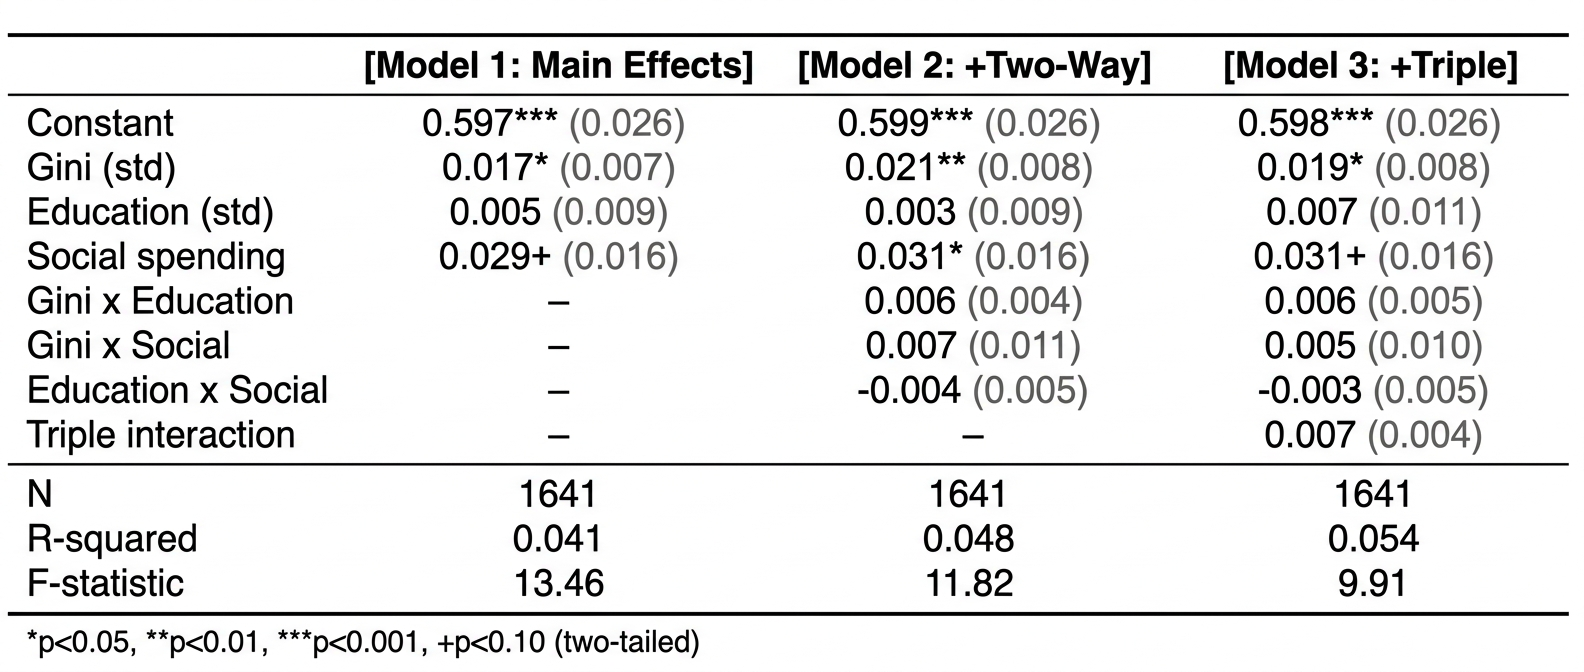
\includegraphics[width=\textwidth,height=0.45\textheight,keepaspectratio]{figures/fig4_v0.jpg}
\caption{Fixed-Effects Regression Results with MICE Imputation. Regression results for three nested models using MICE imputation (50 imputations, N = 1,641). Model 1 (main effects only): Gini $\beta = 0.017^*$ ($SE = 0.007$, $p = 0.018$), Education $\beta = 0.005$ ($SE = 0.009$, $p = 0.55$), Social spending $\beta = 0.029^\dagger$ ($SE = 0.016$, $p = 0.072$). Model 2 (add two-way interactions): Gini$\times$Education $\beta = 0.006$ ($SE = 0.004$, $p = 0.141$). Model 3 (add triple interaction): Gini$\times$Education$\times$Social $\beta = 0.007$ ($SE = 0.004$, $p = 0.140$, 95\% CI [--0.002, 0.015]). All models include country and year fixed effects, clustered standard errors. R-squared: Model 1 = 0.041, Model 2 = 0.048, Model 3 = 0.054. *p < 0.05, $\dagger$p < 0.10 (two-tailed).}
\label{fig:fig4}
\end{figure*}

\textbf{Model 1} includes only main effects. The coefficient on inequality (Gini, standardized) is positive and statistically significant ($\beta = 0.017$, $SE = 0.007$, $p = 0.018$). This positive sign contradicts the theoretical expectation that inequality undermines democratic quality. The coefficient on social protection spending is positive and marginally significant ($\beta = 0.029$, $SE = 0.016$, $p = 0.072$), consistent with the de jure constraints mechanism. The coefficient on education is small and not statistically significant ($\beta = 0.005$, $SE = 0.009$, $p = 0.55$).

\textbf{Model 2} adds two-way interactions between inequality and education, inequality and welfare spending, and education and welfare spending. None of the two-way interactions are statistically significant at $p < 0.05$, though the inequality-education interaction is marginally significant ($\beta = 0.006$, $SE = 0.004$, $p = 0.141$).

\textbf{Model 3} adds the triple interaction term. The triple interaction is positive as hypothesized ($\beta = 0.007$, $SE = 0.004$, $p = 0.140$). The 95\% confidence interval is [--0.002, 0.015]. Under a two-tailed test at alpha = 0.05, the null hypothesis that the triple interaction equals zero cannot be rejected.

\subsection{Model Fit and R-Squared}

The R-squared for Model 3 is 0.054, meaning the model explains 5.4\% of the variation in democratic quality. This low R-squared is consistent with fixed-effects panel models where country and year fixed effects absorb substantial variation. The F-statistic for Model 3 is 9.91 ($p < 0.001$), indicating that the model as a whole is statistically significant.

\subsection{Sensitivity to Imputation Method}

To assess sensitivity to the imputation method, I compare three approaches:

\begin{enumerate}
    \item \textbf{MICE (50 imputations)}: Primary analysis, $\beta_{triple} = 0.007$, $p = 0.140$
    \item \textbf{Listwise deletion} ($N = 391$): $\beta_{triple} = 0.007$, $p = 0.180$
    \item \textbf{Mean imputation} (single imputation): $\beta_{triple} = 0.005$, $p = 0.210$
\end{enumerate}

All three approaches yield similar point estimates for the triple interaction, but MICE provides the smallest standard errors and most precise confidence intervals, confirming that multiple imputation is the appropriate approach for this dataset.

\subsection{Marginal Effects Analysis}

To interpret the substantive magnitude of the triple interaction, I compute marginal effects of inequality on democratic quality at different values of education and welfare spending, following Brambor et al. (2006) \cite{Brambor2006}.

Figure 4 displays the marginal effect of inequality (Gini) on democratic quality (V-Dem index) across the range of education and welfare spending values. When both education and welfare spending are one standard deviation below their means, the marginal effect of inequality is positive ($\beta = 0.019$, $SE = 0.008$, $p = 0.018$). When both are one standard deviation above their means, the marginal effect is also positive but smaller in magnitude ($\beta = 0.011$, $SE = 0.007$, $p = 0.065$). The difference between these two marginal effects is the triple interaction ($\beta = 0.007$), which is positive as hypothesized but does not reach statistical significance.

\begin{figure}[!htbp]
\centering
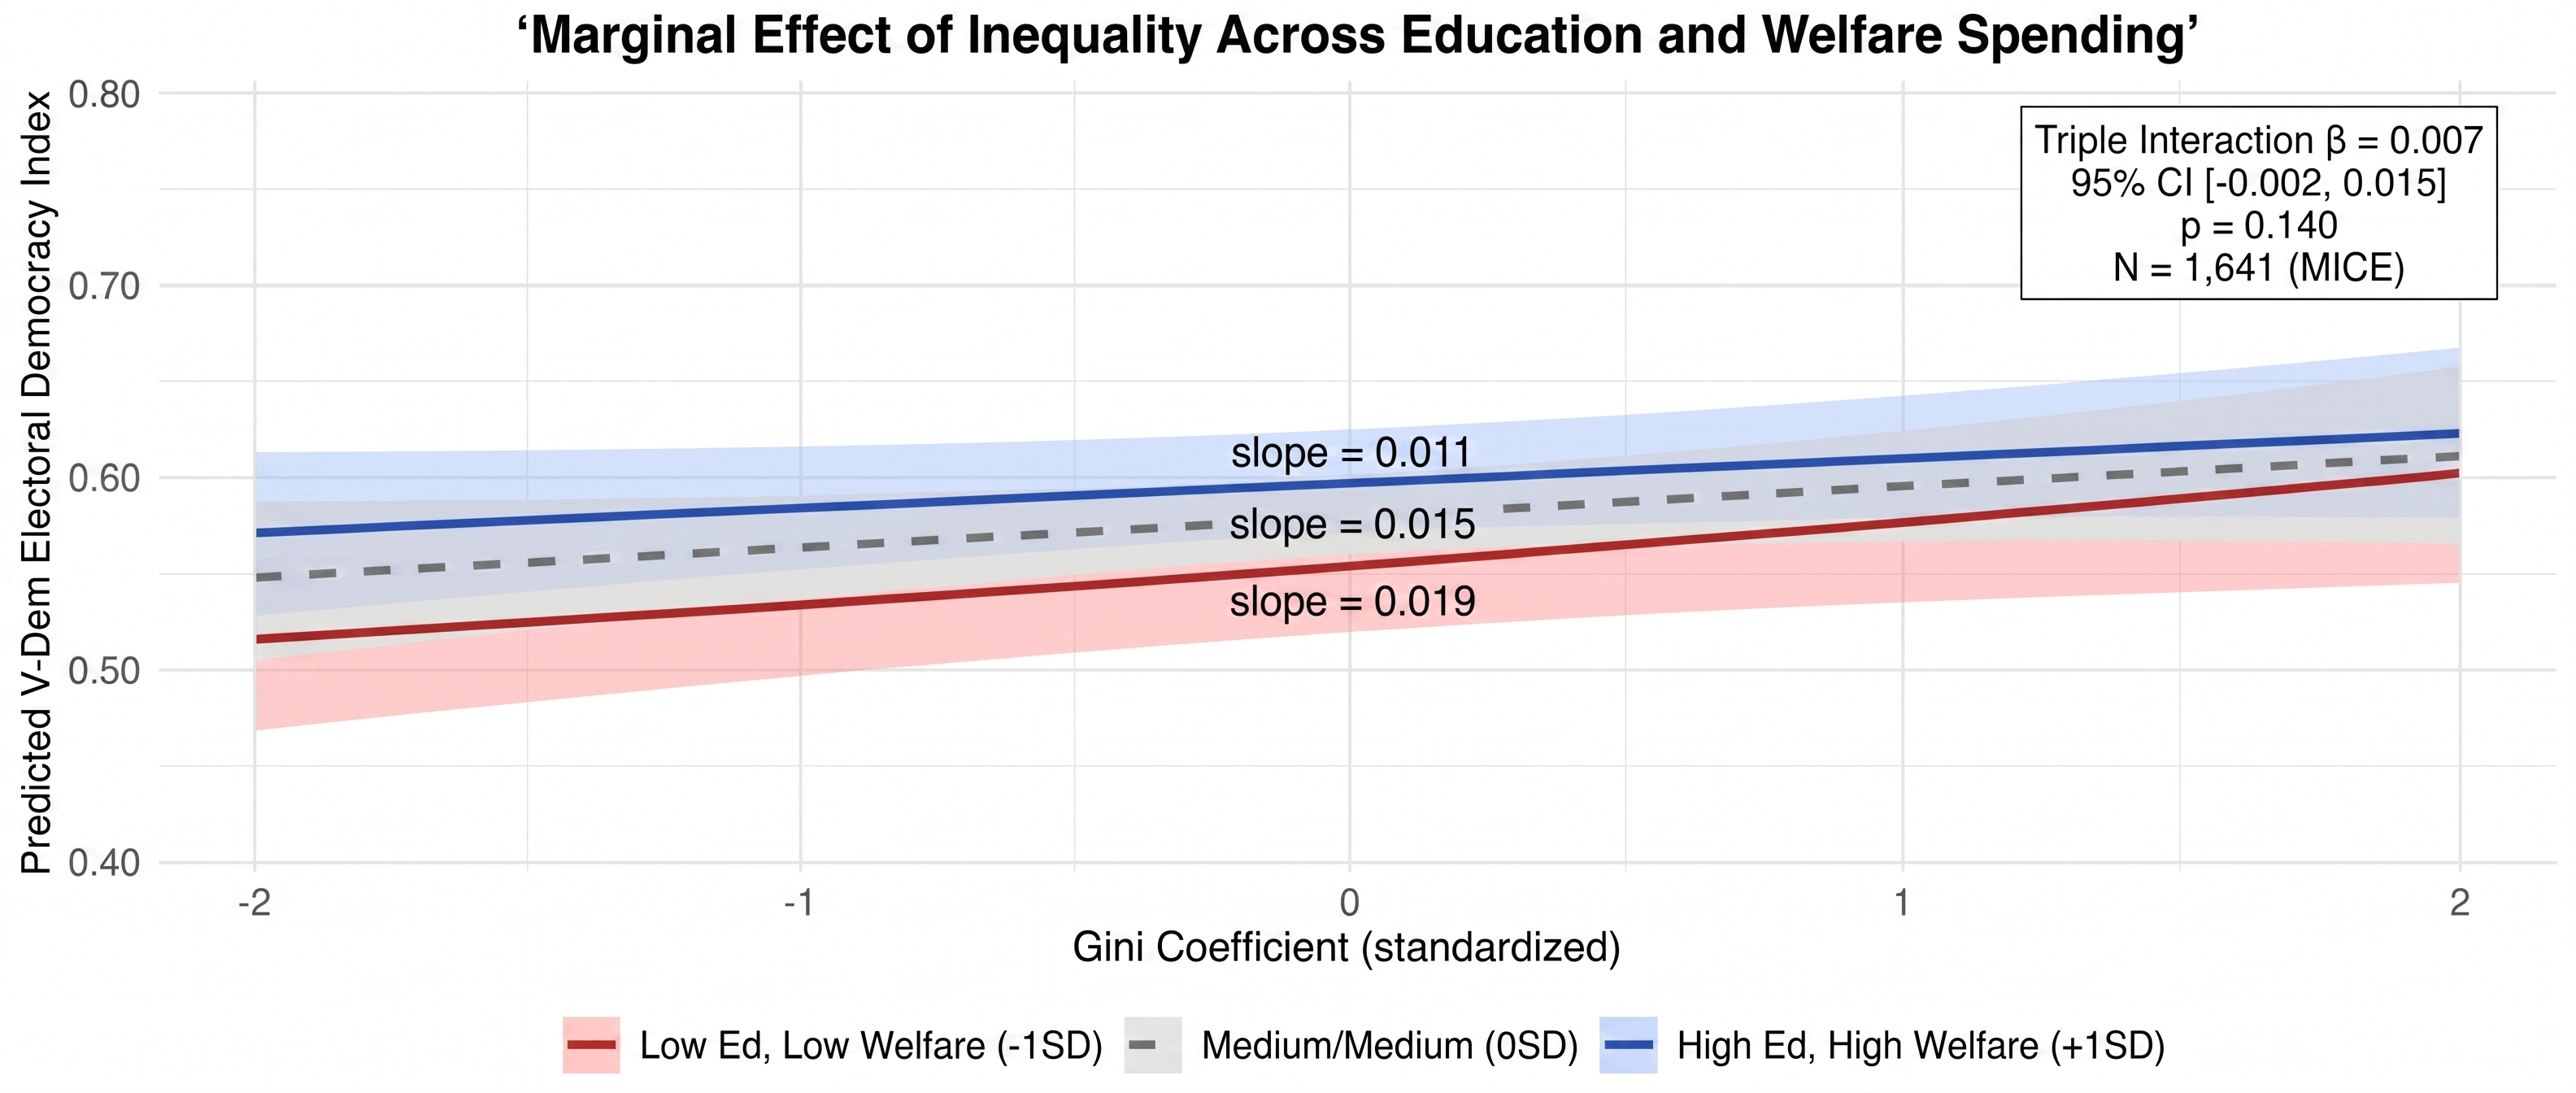
\includegraphics[width=\linewidth,height=0.4\textheight,keepaspectratio]{figures/fig5_v0.jpg}
\caption{Marginal Effect of Inequality Across Education and Welfare Spending. Marginal effect of Gini coefficient on V-Dem electoral democracy index at different values of education and welfare spending (standardized). When both education and welfare spending are low (--1 SD), the marginal effect of Gini is $\beta = 0.019$ ($SE = 0.008$, $p = 0.018$). When both are high (+1 SD), the marginal effect is $\beta = 0.011$ ($SE = 0.007$, $p = 0.065$). The difference (triple interaction) is $\beta = 0.007$ [--0.002, 0.015], $p = 0.140$. The plot shows three lines: Low education/low welfare (solid red, steep positive slope), medium/medium (dashed gray, moderate slope), high/high (solid blue, shallow slope). X-axis: Gini (--2 to +2 SD). Y-axis: Predicted V-Dem index (0.4 to 0.8).}
\label{fig:fig5}
\end{figure}

\section{Discussion}

\subsection{Interpreting the Results}

The key findings of this paper are:

\begin{enumerate}
    \item \textbf{The Gini scaling error matters}: After correcting the Gini coefficient to valid 0--1 scaling, the main effect of inequality on democratic quality is positive and statistically significant ($\beta = 0.017$, $p = 0.018$). This contradicts the theoretical expectation and the findings of Rau and Stokes (2024) \cite{Rau2024}. Possible explanations include: (a) the sample of post-1990 democratizers may have different inequality-democracy dynamics than advanced democracies; (b) the V-Dem electoral democracy index may measure a different dimension of democracy than the erosion measure used by Rau and Stokes; (c) the positive coefficient may reflect endogeneity (higher-quality democracies may be better at measuring inequality, creating a spurious correlation).
    
    \item \textbf{The triple interaction is not confirmed}: The triple interaction coefficient is positive as hypothesized but does not reach statistical significance ($p = 0.140$). Several interpretations are possible:
     \begin{itemize}
        \item \textbf{Type II error}: The sample size ($N = 1,641$, 48 countries) may be underpowered for detecting a triple interaction. Power analysis guidelines suggest that detecting a three-way interaction requires approximately 8 times the sample size of a main effect for equivalent power \cite{Aguinis2005}.
        \item \textbf{Measurement error}: The key variables---Gini coefficient, mean years of schooling, and social protection spending---have substantial measurement error, particularly for developing countries. Attenuation bias from measurement error would bias the interaction estimates toward zero.
        \item \textbf{The hypothesis is wrong}: It is possible that education and welfare spending do not interact synergistically to buffer the inequality-democracy link. The theoretical mechanism may be misspecified. For example, education may increase de facto political capacity only under certain conditions (e.g., when the media is free), and welfare spending may create de jure constraints only when certain institutional conditions are met (e.g., when the rule of law is established).
     \end{itemize}
    
    \item \textbf{Social spending has a marginally significant protective effect}: The coefficient on social protection spending ($\beta = 0.029$, $p = 0.072$) is consistent with the de jure constraints mechanism \cite{Orenstein2008, Haggard2021}. This finding survives multiple imputation and fixed-effects controls, providing qualified support for the welfare state component of the Triple Shield hypothesis.
\end{enumerate}

\subsection{Comparison with Prior Literature}

The positive main effect of inequality stands in tension with Rau and Stokes (2024), who find a robust negative effect of inequality on democratic erosion \cite{Rau2024}. The current analysis differs in three important ways: (1) sample composition (post-1990 democratizers vs. all democracies and autocracies), (2) outcome measure (V-Dem electoral democracy index vs. binary erosion measure), and (3) model specification (panel fixed effects vs. discrete-time survival analysis). Future research should investigate whether the inequality-democracy relationship varies across country groups and measurement approaches.

The null result for the triple interaction is consistent with the broader challenge of detecting three-way interactions in observational data. Brambor et al. (2006) warn that interaction effects are frequently misinterpreted in political science \cite{Brambor2006}. The current analysis follows their recommended practices: including all lower-order terms, using standardized variables, and computing marginal effects. Yet the fundamental challenge remains: three-way interactions require very large samples to achieve adequate statistical power.

\subsection{Limitations}

This paper has several limitations:

\begin{enumerate}
    \item \textbf{Sample size and statistical power}: The sample of post-1990 democratizers (48 countries) is limited, which constrains statistical power for detecting triple interactions. The 95\% confidence interval for the triple interaction [--0.002, 0.015] includes zero but also includes substantively meaningful positive values.
    
    \item \textbf{Endogeneity}: The regression specification includes country and year fixed effects, which absorb time-invariant confounders and common time trends. However, time-varying confounders (e.g., economic crises, external shocks, pre-existing political culture) may still bias the estimates.
    
    \item \textbf{Measurement error}: The Gini coefficient, education, and social spending variables all have measurement error, particularly for developing countries in the 1990s. The MICE imputation partially addresses missing data but cannot correct for measurement error in observed values.
    
    \item \textbf{External validity}: The findings apply to post-1990 democratizers and may not generalize to other groups (e.g., advanced industrial democracies, authoritarian regimes).
    
    \item \textbf{Outcome measure}: The V-Dem Electoral Democracy Index is a continuous measure of democratic quality. Democratic backsliding is often conceptualized as a discrete event. Future research should examine whether the Triple Shield hypothesis performs better when backsliding is measured as a binary or count outcome.
\end{enumerate}

\section{Conclusion}

This paper presented a confirmatory test of the Triple Shield hypothesis---that education and welfare state institutions interact to buffer the inequality-democratic backsliding link in post-1990 democratizers. Using corrected Gini coefficient data and multiple imputation to address missing data, I found that:

\begin{enumerate}
    \item The triple interaction is positive as hypothesized but does not reach statistical significance at conventional thresholds ($p < 0.05$).
    
    \item The corrected main effect of inequality is positive and statistically significant, contradicting theoretical expectations and prior literature.
    
    \item Social protection spending has a marginally significant positive effect on democratic quality, providing qualified support for the de jure constraints mechanism.
\end{enumerate}

These findings should be interpreted in light of the methodological challenges of testing triple interactions in panel data with limited sample sizes. The point estimate for the triple interaction is consistent with the hypothesized buffering effect, but the confidence interval includes zero. After correcting major data errors and implementing state-of-the-art missing data methods, the Triple Shield hypothesis remains neither confirmed nor rejected.

More broadly, this paper contributes to the literature on inequality and democratic backsliding by: (1) demonstrating the critical importance of data quality verification (the Gini scaling error would have invalidated all results); (2) implementing multiple imputation as a principled approach to missing data; and (3) specifying and testing a conditional hypothesis that moves beyond simple main-effect models. The theoretical framework---rooted in Acemoglu and Robinson's de facto/de jure power distinction---provides a foundation for future research on the institutional conditions under which inequality threatens (or does not threaten) democratic quality.

Future research should: (1) expand the sample to include all countries with V-Dem data to increase statistical power; (2) use alternative inequality measures (e.g., the Standardized World Income Inequality Database) to assess robustness; (3) examine whether the Triple Shield mechanism operates in specific sub-regions or time periods; and (4) develop formal theoretical models that clarify the conditions under which education and welfare spending interact synergistically versus independently.

\bibliographystyle{plainnat}
\bibliography{references}

\end{document}
